\chapter{Introduction}
\label{chp:intro}
Huge amounts of data are generated in an unprecedented rate nowadays from different application domains like social networks, telecommunications, WWW, scientific experiments, e-commerce systems, health care systems, etc. These data flow in and out of systems continuously, but with varying update rates. For example, banking systems register each of their ATM and account transactions, telecommunication providers log each of their calls' information, popular websites maintain their user logging details, organizations like CERN produce petabytes of data during their experiments; these are known as stream data. The volume and the rate of incoming data make it nearly impossible to mine these data with traditional data mining approaches. As alternatives, mining a subsample of the data or mining for much simpler models can be some options. This, however, drastically limits the ability to extract information from the data. Moreover, in some cases, accumulating and storing the data during runtime, and performing a sampling to apply mining algorithms simultaneously is a challenge. For such reasons the notion of mining fixed-size databases is slowly being replaced by the idea of mining open-ended data streams.

Compared to the classical data mining approaches stream mining is relatively a new topic. Even though for batch approaches both classification and clustering problems have been vastly studied, their stream adaptations remain a challenge due the restrictions imposed by the stream data. In particular, due to the volume and the nature of the stream data there are several restrictions that are needed to be considered while designing a stream mining algorithm. Most important limitations include not being able to store the complete data set in memory, and hence only being able to use an example once to train the model; evolving nature of the data with time changes, etc. Thus stream mining requires a different approach than the traditional batch learning. The possibility of temporal locality makes the classification problem even harder in a streaming environment. Algorithms need to address the evolution of the underlying data stream.

Traditional machine learning algorithms generally feature a single model, e.g. Na\"ive Bayes or multilayer perceptron (MLP) learned from a training set and use it to classify a testing set. The parameters of these learners (e.g., weights of a feed-forward neural network) are set by realizing the complete training set. These classifiers provide a measurement of the generalized performance, i.e., how well the classifiers generalize the training set. Some of the assumptions that these algorithms make are: (i) data are finite, (ii) underlying data regularities are stationary, (iii) stationary data sources generate independent and identically distributed data, (iv) data are invariant to the spatial or temporal changes, etc. However, none of these assumptions is valid for data streams. Stream data exhibit the following characteristics: 
\begin{itemize}
    \item Data come as a continuous flow of an unlimited stream, often at a very high speed.
    \item Underlying models in the data evolve over time.
    \item Data cannot be considered to be independent and identically distributed.
    \item Time and space can significantly influence data.
\end{itemize}
At the first glance, it may seem that some simple adaptation of current methods should be sufficient to address these characteristics. In reality though, these changes challenge most trivial learning methods of machine learning, for example, entropy computation. For batch learning, all the instances and their corresponding classes are known before-hand to compute entropy. However, for the streaming case, a data stream is no longer finite, the number of classes are not known a priori, and the domains of variables are not necessarily small in size. Hence, the computation of batch-like entropy function is not possible. Similarly, maintaining a frequent item sets over hundreds of gigabytes of a database cannot be easily supported by traditional machine learning algorithms.

Adaptations of traditional algorithms need to address the continuous flow of data, the dynamic environment of generating sources, and the unavailability of a complete data set, etc. Some of the new requirements that are needed to be considered while developing a knowledge discovery system for stream data are listed below:
\begin{itemize}
    \item Algorithms should use limited resources, e.g., memory and processing time.
    \item Algorithms should only access the data a limited number of times, and may only use a limited bandwidth.
    \item Algorithms should always be able to predict. That is, irrespective of the number of the training instances, the algorithms should be able to classify a new instance.
    \item Data gathering and processing might be distributed.
\end{itemize}

With traditional algorithms, a single model is typically learned, i.e. only one single generalization of the data is learned. However, given a finite set of training examples, it is rather reasonable to assume that the data might contain several generalizations. For example, a different initial setting of a neural network classifier (weights, node layers, node counts, etc.) might change the final network to some extent. For stream environment this assumption becomes primitive. Thus, choosing a single classifier is not always optimal. Using the best classifier among several classifiers, where each is trained with the same training set, would be an alternative; however, information is still being lost by discarding sub-optimal options. A better alternative would be to build a classifier ensemble. Ensemble classifiers combine the predictions of multiple base level models. A simple process for combining base model predictions would be majority voting. As demonstrated in several works~\cite{breiman94:bagging, schapire90:whyens} such ensemble methods (e.g. ensembles of neural networks) yield better performance as compared to the non-ensemble methods.

However, without proper selection and control over the training process of the base learners, ensemble classifiers could result in poorer performance. Simply choosing a base classifier and training it for several settings would surely produce highly correlated classifiers which would have adverse effect on the ensemble performance. One solution of this issue is to train each classifier with its own training set generated by random sampling over the original training set. However, with random sampling each classifier would receive a reduced number of training instances, resulting in a reduction in the accuracy of the individual base classifiers. This reduction in the base classifiers' accuracy is generally not recovered by the gain of combining the classifiers unless measures are taken to make the base classifiers diverse.

Diversity is generally achieved by making the base classifiers minimally correlated. In recent years, various methods have been developed to address this issue, e.g., bagging, and boosting. Some of these approaches are suitable for label based classification, and some can be used to approximate the trend of data over a specific time granularity. It would, however, be nice if a method can approximate the trend of data over a set of time granularity. Moreover, how the ensemble methods perform where base classifiers are trained to predict one specific label should be interesting to investigate. For example, given a Twitter stream an ensemble of classifiers that may contain base classifiers to classify sentiments for sports, politics, entertainment, etc. separately. It is expected that this ensemble setting would out-perform the generic ensemble approach over the complete stream.

Ensemble methods build model outputs where abstract properties of the algorithms that produces the model are prioritized rather than the specifics of the algorithms. This allows a wide application across many fields of study. With precise use of ensemble methods, it would be possible to automatically exploit the strengths and weaknesses of different machine learning systems.

This thesis investigates such existing ensemble approaches for data streams, and presents an empirical analysis of those methods. Moreover, this thesis presents a unique perspective in respect to the underlying setup that generates the stream, which applies to certain application domains such as social media. In the following sections, we present this motivation and probable approaches to address such scenarios.

%\newpage
\section{Motivation}
\label{sec:intro:motiv}
One of the major challenges faced in stream mining is the lack of labeled data. In batch learning, data are finite and generally a high percentage of data is labeled. Some semi-supervised learning methods can be used, if some labels are missing. Streaming scenarios show a stark contrast, as most of the real world data are (mostly) unlabeled. It needs human intervention, resources, and time to properly label a stream data set. Most often only a fraction of a data set is labeled by human experts or through automated scripts. Because of such limitations, a large number of experimentations for stream mining algorithms are performed using synthesized data. Also, it is much easier to control different parameters like concept drift, labeling, etc. in a generated data set. In most of the approaches, this data generation process is mostly randomized, and the originating of data generating from a certain region remains the same for the entire hyperspace. Temporal locality is sometimes created by adding bias to certain region, however, the rates at which these regions produce data points mostly remain the same for all the regions in the hyperspace.

In reality many practical scenarios do not follow a uniform distribution for data generation. Rather, some regions are more active than others. The term ``more active'' here means that they produce more data. For example, Figure~\ref{fig:intro:nettraffic} shows the Internet traffic on an average day. A reference heat-map scale is given where the blue color represents less than average and red represents higher than average. As the figure shows based on the time of the day, the amount of network traffic in each region changes drastically even though the number of active nodes remains almost the same.

\begin{figure}[htbp] 
    \begin{center}
        \begin{tabular}{cc}
            \resizebox{70mm}{!}{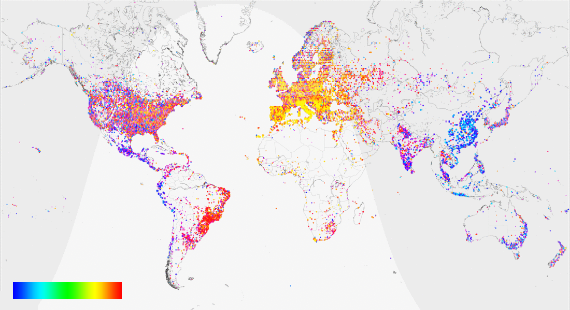
\includegraphics{figs/nettraffic-a.png}} &
            \resizebox{70mm}{!}{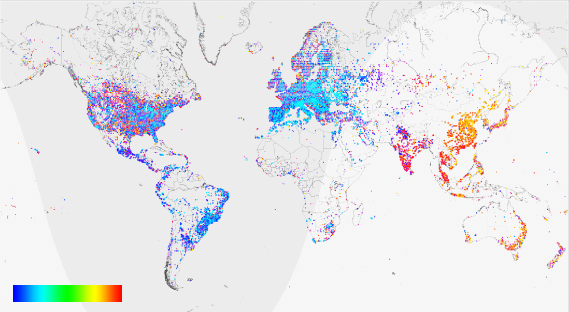
\includegraphics{figs/nettraffic-b.png}} \\
            \scriptsize{(a)\vspace{2mm}} &
            \scriptsize{(b)}    
        \end{tabular}
        \caption{Worldwide Internet traffic~\cite{internet:huffpost:nettraffic}. Daytime Internet usage in (a) western (b) eastern hemisphere}
        \label{fig:intro:nettraffic}
    \end{center}
\end{figure}

As another example, let us consider profiling of phone users based on the phone usages. Typically, young people are more inclined towards using data services rather than voice services while professionals and elderly people mostly use voice services. Thus, the profiling algorithm should consider these differences in rates in which different user groups are using the services.

To get a clearer picture of the locality of data activation and rate in which data are generated, let's consider the social media statistics. As of the second quarter of 2015, Facebook had 1.49 billion monthly active users. In the third quarter of 2012, the number of active Facebook users had surpassed 1 billion. Active users are those who logged into Facebook during the last 30 days. It was only on the August 28, 2015, that Facebook had 1 billion users on a single day. Let us assume that we want to do a sentiment analysis over the data collected from a week of activity in Facebook. Even though the class distribution (positive and negative sentiments)  may remain balanced, however, more active users will clearly ``overshadow'' the inputs given by the less active users. Similarly, about 300 million users produce 500 million tweets per day on Twitter. Figure~\ref{fig:intro:tweets} shows tweets for 5 different hashtags, namely, \#Trump, \#Syria, \#football, \#Volkswagen, and \#eclipse for the period of Aug 29, 2015 - Sept 28, 2015 (\cite{internet:topsy:tweets}). 
\begin{figure}[htbp] 
    \begin{center}
            \resizebox{110mm}{!}{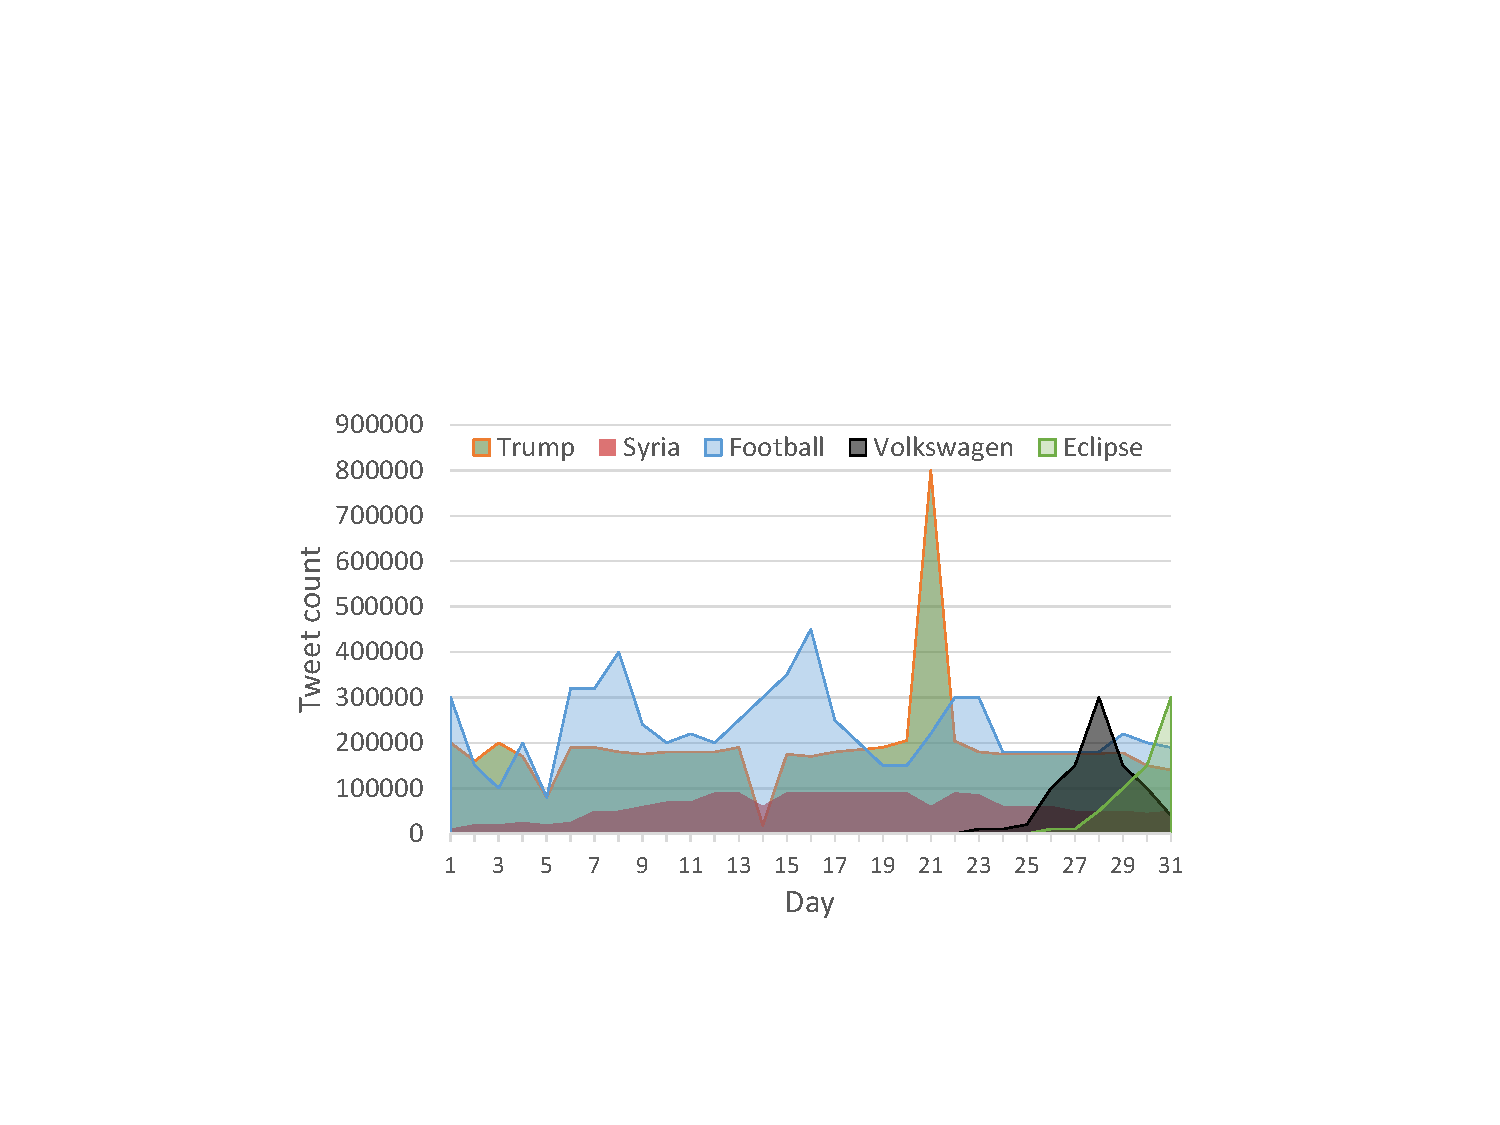
\includegraphics{figs/tweets.pdf}}
        \caption{Number of tweets for different hashtags }
        \label{fig:intro:tweets}
    \end{center}
\end{figure}
\noindent As it can be seen, \#football has a weekly repetitive trend, most certainly because of weekend games. \#Trump (USA's presidential candidate for 2016), on the other hand, has a steady rate with occasional spikes depending on some highlighted events, e.g., debate. The topic \#Syria has lower rate, however, it has a steady flow. Owing to the news of carbon emission from Volkswagen cars and lunar eclipse of September 28, 2015, topics like \#Volkswagen and \#eclipse got trending, however, they are expected to disappear soon. If each of these topics is to be treated equally, slower but consistent streams like \#Syria would suffer from lack of data volume. 

Based on the discussion above, it is evident that these streams do not necessarily follow a uniform distribution. Rather, these streams can be considered as a collection of many sub-streams, with following properties:
\begin{itemize}
    \item Slow sub-streams generating low but relatively consistent number of data, e.g., \#Syria.
    \item Alternating sub-streams generating moderate number of data. Activation of sub-streams within the set is dependent on each other, e.g., streams related to the football clubs.
    \item Sub-streams that produce a very large amount of data but remain active for only very short periods of time, e.g., \#eclipse.
\end{itemize}

Applying machine learning methods in such streams without considering the differences in the rate of data incoming from different sub-streams might lead to a set of decision rules dominated by the sub-streams with the highest number of instances. Moreover, most stream mining algorithms only keep track of most recent incoming instances and forget older data. Such algorithms would thus forget important decision rules learned over longer periods of time for slow but consistent sub-streams when a heavy burst of occasional sub-streams arrives. It would take a long time to learn the same rules again. Similarly, a burst could lead to the deletion of decision rules for recurring sub-streams too. This could significantly affect the performance of the models. Even for slow sub-streams the overall performance measures may not reflect poor decision performances for those slow sub-stream, as the number of instances belonging to those streams is not high. But, ideally we would expect that the mining algorithms should be effective for the entire data space.

In this thesis, we address such scenarios. To the best of our knowledge no previous work has specifically addressed this issue. In most works, the evaluation is performed with randomized streams, and concept drift, concept evolution, concept recurrence, etc. are addressed within the randomized stream. We extend one such data generation algorithm to implement the scenario presented above. Empirical evaluation is performed to compare the performances of existing algorithms for such streams. Comparing the results with the results from general randomized streams, it is found that existing algorithms do not perform at their best for streams with high temporal locality. Thus, this thesis presents an ensemble algorithm derived from one of the state-of-the-art algorithms to improve its performance in such scenarios. Extensive evaluation shows that the new method achieves more stable results and overcomes the challenges posed by the nature of the stream. It also retains all the positive factors of the original algorithm.

The next section discusses the basic idea of the algorithm without going into mathematical details. We present the algorithm later in great detail once the related literature and the concepts are introduced in the next couple of chapters.

\section{Intuition}
\label{sec:intro:intu}
The central idea of our method is based on the primal decision tree adaption by Domingos and Hulten~\cite{domingos00:vfdt} for streams named Very Fast Decision Tree (VFDT), also commonly known as Hoeffding Tree (HT). Their method is based on the assumption that to find the best attribute for a split decision at any node in a decision tree, it would be sufficient to consider only a certain amount of training data on that node. The Hoeffding bound~\cite{hoeffding63:bound} is a measurement for the degree of certainty for such an approach, which gives an error bound for a decision taken after seeing a certain amount of instances. This bound essentially states that any decision taken after observing a certain amount of instances would remain the same after seeing an infinite number of instances and the error margin can be computed with this bound. A detailed discussion of this bound and the algorithm is presented in Chapter~\ref{chp:background}.

With such an approach, challenges posed by high volumes of data can be avoided as we do not need to remember all the observed data instances. Rather, the statistics of the instances are sufficient to effectively decide about a split attribute. One of the limitations of a Hoeffding Tree is that it grows linearly as the time passes or as the instances arrive in the system. The root of the tree is the node that is used for splitting the oldest set of examples. Similarly, decision rules at lower levels also become old, while the leaves contain information from the most recent instances. To keep the rules updated numerous approaches such as resetting the tree, pruning bad performing nodes, etc., have been proposed. A detailed discussion of adaptations for concept drift, evolution, recurrence, etc. is presented in Chapter~\ref{chp:background}.

With the reset and pruning property, the Hoeffding Tree exhibits a special property, in particular. It always adapts itself for the newer examples. The number of examples upon which the HT's decision rules depend on is directly related to the size of the tree and the number of examples required to split a node. The number of decision or split nodes could be a measurement of the size of the tree. A smaller tree would adapt faster to the changes in the data, whereas, a larger tree would take longer time to adapt. Using this rationale a bagging method based on different sized trees is proposed by Bifet et al.~\cite{bifet09:asht}. In this method, a fixed number of Hoeffding Trees with different size (number of decision nodes) limits are used. Each time a tree exceeds the size threshold, the tree gets reset. Trivially, smaller trees would reset more often than the larger trees, and thus, the decision rules from smaller trees will base on the most recent data. Larger trees, however, would contain decision rules from older data.

We combined these concepts to address our problem. First, we introduced a size restricted variant of Hoeffding Tree named Size Restricted Hoeffding Tree (SRHT). Unlike its predecessor Adaptive Size Hoeffding Tree~\cite{bifet09:asht}, SRHT does not get reset immediately after it reaches the size limit. Instead, it stops growing i.e. no further split occurs, however, the weights in the leaf nodes are updated with incoming instances. It also combines two different concepts introduced by its predecessors: (i) it resets once a size limit is reached and (ii) it maintains alternate trees or subtrees when necessary. Thus, even after reaching the size limit, a tree can switch to its alternate tree and start growing again. This ensures that the model would remain updated to some extent in a drifting environment, even though the tree growth would be restricted.

We use this setup in a modified bagging scheme introduced in~\cite{bifet09:asht}. Similar to the Hoeffding Tree, a smaller SRHT will have decision rules for most recent data, and a larger tree would contain rules for some older instances, too. In our problem's context, a smaller tree would have decisions for high speed sub-streams or burst of incoming streams. Whereas only the larger trees will have some decision rules for slow but consistent sub-streams, along with the decision rules for most recent data. This is because, the recent data are always dominated by high speed sub-streams. Smaller data portions do not contain enough information about the slow streams or enough examples from slow streams to decide on them. Keeping this in mind, we control the reset of larger trees to keep hard-learned decision rules (hard in terms of time required). In doing so, we maintain an alternate pool of trees that are to be reset soon, and we start to maintain a new tree with same size limit from scratch. For the transition time we consider votes from all the trees, thus effectively increasing the weights for slower streams. In Chapter~\ref{chp:algo}, we present more elaborate description of the proposed approach.

\section{Related Works}
\label{chp:relworks}
Compared to data mining, stream mining is a young area. Most of the methods date back only a couple of decades. Similarly, the concept of ensemble learning was first introduced in the traditional batch learning, however, ensemble adaptations for streams are fairly new concepts. In this chapter, we list the most influential methods developed so far with particular focus on tree based learners. We follow a rudimentary narrating style starting directly with methods for general stream learners for stationary streams, and then for evolving data streams. After that, we list the base methods for ensemble learning, and finally we present ensemble based stream learners.

\subsection{Stream Mining}
%Compared to the classical data mining approaches stream mining is relatively a newer topic to be addressed in literature. Even though for batch approaches both classification and clustering problems have been vastly studied, their stream adaption remains a challenge due the restrictions imposed by the stream data. Possibility of temporal locality makes the classification problem harder in a streaming environment. Algorithms needs to address the evolution of underlying data stream. 

Domingos and Hulten introduced a strict one-pass adaptation of decision tree approach~\cite{breiman84:dt,quinlan93:c45} for data streams. Classic approaches like ID3 and C4.5 learners assume that all training examples can be stored in the main memory altogether. This is a significant limitation to the number of examples these algorithms can handle. Similarly, disk based decision tree learners (SLIQ~\cite{mehta96:sliq}, SPRINT~\cite{shafer96:sprint}, etc.) become very expensive when data sets are very large and the expected trees has many levels. Domingos and Hulten proposed \textit{Very Fast Decision Trees (VFDT)}~\cite{domingos00:vfdt} that uses the Hoeffding bound~\cite{hoeffding63:bound} to build an anytime decision tree for constant memory and time. The primary assumption in this approach is that to find the best attribute for a node in a decision tree, it may be sufficient to consider only a fraction of the training set that passes through that node. The Hoeffding bound provides a statistical measure to determine how much data is needed to ensure a level of degree of certainty, i.e. the error margin would be bounded by a given value~\cite{catlett91:thesis}.

Like most statistical and machine learning algorithms VFDT assumes that training data is randomly drawn from a stationary distribution. This assumption is not valid for large databases and data streams. Over time an underlying method or environment that generates data could change. The shift is  referred to as {\it concept drift} in the literature and can be abrupt as well as very slow. Data related to weather forecast, economic condition prediction, mis-calibrated sensors, etc. are examples of a concept drifting environment. A concept-adaptive variant of VFDT, \textit{CVFDT}~\cite{hulten01:cvfdt}, can handle such scenarios. CVFDT updates its decision rules, essentially the tree structure, by detecting the concept drift in the data. It maintains alternate subtrees whenever an old subtree becomes questionable, and replaces the old one with the alternative when it becomes more accurate. CVFDT uses a sliding window and updates sufficient statistics by increasing the count of newly arrived examples and decreasing the count of old examples in the window. Essentially CVFDT achieves same accuracy that would be achieved if VFDT had been run again with the new data. CVFDT does this in $O(1)$ time with an additional space requirement as compared to the VFDT's $O(w)$ complexity where $w$ is the window size. Another extension of VFDT, VFDTc was proposed in~\cite{gama05:vfdtc} that improves VFDT by handling continuous numeric attributes and adding na\"ive Bayes prediction at the leaves of the tree.


% TODO: briefly include multi-label evolving ...
% TODO: frequent item set mining]

\subsection{Ensemble Learning}
Traditional machine learning algorithms generally feature a single model or classifier such as \textit{na\"ive Bayes} or \textit{multilayer perceptron (MLP)}. The free parameters of these learners (e.g. weights of feed-forward neural network) are set by realizing the complete training set. These classifiers provide a measurement of the generalization performance i.e. how well the classifier generalizes the training set. However, given a finite set of training example, it is rather reasonable to assume that the data might contain several generalizations. For example, a different setting of the neural network classifier (weights, node layers, node counts, etc.) changes the final network to some extent. For stream environment, this assumption becomes trivial. Thus, choosing a single classifier is not always optimal. Using the best classifier among several classifiers where each is trained with the same training set would be an alternative, however, information is still being lost by discarding sub-optimal options. A better alternative would be to build a classifier ensemble. Ensemble classifiers combine the prediction of multiple base level models built on traditional algorithms. A simple process for combining the predictions could be to choose the decision based on majority voting~\cite{parhami94:voting}. As demonstrated in several works~\cite{breiman93:regression, schapire90:whyens, wolpert92:whyens}, ensemble methods (e.g. ensembles of neural networks)~\cite{hansen90:ensNN, tumer99:whyens} yield better performance. 

Without proper selection and control over the training process of the base learners, ensemble classifiers could result in poorer performance. Simply choosing a base classifier and training it for several settings would surely produce highly correlated classifiers which would have adverse effect on the overall ensemble process. One solution of this  is to train each classifier with its own training set generated by random sampling of the original one. However, with random sampling each classifier would receive a reduced number of training patterns, resulting in a reduction of the accuracy of the individual base classifier. This reduction in the base classifier accuracy is generally not recovered by the gain of combining the classifiers unless measures are taken to make the base classifiers \textit{diverse}. Classifiers with complementary information would give the lowest correlation~\cite{breiman93:regression, tumer99:whyens}. Many methods have been proposed to promote diversity among the base classifier: \textit{bagging}~\cite{breiman94:bagging}, \textit{boosting}~\cite{drucker94:boosting, freund97:boosting, oza99:whyens}, \textit{cross-validation partitioning}~\cite{krogh95:ensNNcv, tumer99:whyens}, etc. These methods mainly process the entire training set repeatedly and require at least one pass for each base model. This is not suitable for streaming scenarios. Stream adaptation of bagging and boosting methods has been introduced by Oza et al.~\cite{oza01:obagboost,oza01:thesis}.

\subsection{Ensemble Learning in Streams}
Learning algorithms in data streams require maintenance of a set of hypotheses based on the training instances seen thus far with the need for storage and reprocessing. Facilitating this requirement, Oza and Russell developed an online version~\cite{oza01:obagboost, oza01:thesis} of traditional bagging and boosting. Bagging works by randomly sampling with replacement from the training set to form a given number of intermediate training sets which are used to train same number of classifiers. During testing a majority voting scheme is employed on the decisions of all classifiers to deduce the final decision. Boosting uses an iterative procedure to adaptively change the distribution of training data by focusing more precisely on misclassified instances. Initially all instances have equal weights, and at the end of a boosting round the weight of each instance is updated by increasing or decreasing if the instance was classified wrongly or correctly, respectively. For the \textit{online} variant of these algorithms, not knowing the size of the training data poses a problem in determining the size of training sets to build the base models. In~\cite{oza01:obagboost} the authors address this situation by training $k$ models with each instances where $k$ is a suitable Poisson random variable. Later on,~\cite{pelossof08:boosting} proposed the \textit{Online Coordinate Boosting} algorithm where the number of weight updates of~\cite{oza01:obagboost} is reduced using few simple alterations.


As mentioned in the previous section, a \textit{Hoeffding Tree (HT)} i.e. VFDT~\cite{domingos00:vfdt}, can be used to build classifiers for concept drifting streams. The Hoeffding Tree has the property that it adapts itself for the newer examples. The number of examples that a HT is built upon is determined by two numbers: (i) the  size of the tree, and (ii) the number of examples used to create a node. Thus, smaller trees adapt faster to the changes in the data, while larger trees try to retain the rules that reflect longer time-frame, simply because they are built on more data. In other words a tree bounded by size $n$ would be reset twice as often as tree bounded by size $2n$. \textit{Adaptive Size Hoeffding Tree (ASHT)} bagging~\cite{bifet09:asht}, uses this intuition to build an ensemble of classifiers of different sized Hoeffding trees. ASHT bagging attempts to increase the diversity in the bagging approach. The maximum allowed size for the $n$-th tree is twice the size of the $(n-1)$-th, where the first tree has a size of $2$. Additionally, the inverse of the squared errors have been used as the weights for the trees. Authors made an observation that bagging using 5 trees of different size might be sufficient to gain higher accuracy, as the error level for bagging with more trees does not improve much but takes longer time.

Same authors also proposed an adaptive window size bagging method-- \textit{ADWIN}~\cite{bifet09:asht}. ADWIN automatically detects and adapts to the current rate of change. To do so ADWIN adapts its window size to maximize the statistically consistently length that conforms following hypothesis ``there has been no change in the average value inside the window''. The window is not maintained explicitly, rather using a variant of an exponential histogram technique that takes $O(log\;w)$ memory and $O(log\;w)$ processing time where $w$ is the length of the window. Experimental evaluation showed that ADWIN bagging has better accuracy than ASHT bagging, however, requires more time and memory. 

ADWIN has later been used in \textit{leverage bagging}~\cite{bifet10:levbag}. Leverage bagging improves randomization by increasing the re-sampling and using output detection codes. Re-sampling with replacement is done in online Bagging using Poisson(1)~\cite{oza01:obagboost}. Instead leverage bagging increases the weights of re-sampling using a larger value $\lambda$ to compute the value of the Poisson distribution. The Poisson distribution is used to model the number of events occurring within a given time interval. Randomization is added at the output of the ensemble using output codes. This method works by assigning a binary string of length $n$ to each class and building an ensemble of $n$ binary classifiers. Each of the classifiers learns one bit for each position in the string. A new instance is classified to the class with the closest binary code. 

ADWIN has also been used in building ensembles of \textit{Restricted Hoeffding Trees}~\cite{bifet10:rht}. A mechanism for setting the learning rate of perceptrons in the base neural network learner using the ADWIN change detection method is used to restrict the tree. Additionally, a mechanism for resetting a member tree is also been introduced when a particular member is no longer performing well. The method outperforms traditional bagging in terms of accuracy, but requires additional memory and time.



\section{Thesis Objectives}
The primary objective of this thesis is to devise an algorithm realizing the intuitions discussed earlier. In doing so, an extensive survey of existing literature is performed. The most relevant portion of which has already been discussed in the previous section. The remaining is attached at the end of the thesis (see Appendix~\ref{appndx:erw}). This thesis presents a new way to look at the composition of various real-world streams e.g. social networks. Based on that, a new approach of data generation to facilitate slow, fast, burst, recurrent, etc. behavior in a randomized data stream is proposed. In an effort to combine the ideas of Adaptive Size Hoeffding Tree and Adaptive Hoeffding Tree using ADWIN, a new ensemble method is devised aiming to improve the performance of slower streams. Lastly, a comprehensive empirical comparison of current Hoeffding tree-based approaches is performed.


\section{Outline}
The rest of the article is organized as follows: Chapter~\ref{chp:background} presents the base concepts required for the thesis. We first discuss the basic streaming adaptations of batch methods, and later their usages in ensemble approaches. Chapter~\ref{chp:algo} precisely defines the problem and discusses the development of our algorithm addressing the motivation and intuition of this chapter. In Chapter~\ref{chp:dataset} existing data set generators are discussed first and a new data generation scheme is explained that fulfills the requirements discussed in the intuition section (Section~\ref{sec:intro:intu}). Finally, before concluding the thesis in Chapter~\ref{chp:conclude}, in Chapter~\ref{chp:exp} we describe the experimental evaluation process and findings. Extensive evaluation is performed to compare existing methods, as well as, the newly developed method. 
